\documentclass[a4paper,14pt]{extarticle}
\usepackage[utf8]{inputenc}
\usepackage[russian]{babel}
\usepackage{graphicx}
\usepackage{indentfirst}
\usepackage[top=0.8in, bottom=0.8in, left=0.8in, right=0.8in]{geometry}
\usepackage{pgfplots}
\usepackage{amsmath}
\usepackage{setspace}
\usepackage{titlesec}
\usepackage{pdfpages}
\usepackage{subcaption}
\usepackage{float}
\usepackage{longtable}
\usepackage{chngcntr}
\usepackage{pgfplots}
\usepackage{amsfonts}
\usepackage{hhline}
\usepackage{pgfplotstable}
\usepackage{multirow}
\usepackage{tikz,xcolor}
\usepackage{listings}

\lstset{ %
extendedchars=\true,
keepspaces=true,
language={[x86masm]Assembler},					% choose the language of the code
basicstyle=\footnotesize,		% the size of the fonts that are used for the code
numbers=left,					% where to put the line-numbers
numberstyle=\footnotesize,		% the size of the fonts that are used for the line-numbers
stepnumber=1,					% the step between two line-numbers. If it is 1 each line will be numbered
numbersep=10pt,					% how far the line-numbers are from the code
backgroundcolor=\color{white},	% choose the background color. You must add \usepackage{color}
showspaces=false, 			% show spaces adding particular underscores
showstringspaces=false,			% underline spaces within strings
showtabs=false,					% show tabs within strings adding particular underscores
frame=single,           		% adds a frame around the code
tabsize=4,						% sets default tabsize to 2 spaces
captionpos=b,					% sets the caption-position to bottom
breaklines=true,				% sets automatic line breaking
breakatwhitespace=false,		% sets if automatic breaks should only happen at whitespace
escapeinside={\%*}{*)},			% if you want to add a comment within your code
%postbreak=\raisebox{0ex}[0ex][0ex]{\ensuremath{\color{red}\hookrightarrow\space}}
}

\titleformat{\section}[hang]
  {\bfseries}
  {}
  {0em}
  {\hspace{-0.4pt}\large \thesection\hspace{0.6em}}
  
  
\titleformat{\subsection}[hang]
  {\bfseries}
  {}
  {0em}
  {\hspace{-0.4pt}\large \thesubsection\hspace{0.6em}}
  
\titleformat{\subsubsection}[hang]
  {\bfseries}
  {}
  {0em}
  {\hspace{-0.4pt}\large \thesubsubsection\hspace{0.6em}}

%\linespread{1.3} % полуторный интервал
%\renewcommand{\rmdefault}{ftm} % Times New Roman

\counterwithin{figure}{section}
\counterwithin{equation}{section}
\counterwithin{table}{section}

\begin{document}
\begin{titlepage}
\centering
Санкт-Петербургский политехнический университет Петра Великого \\
Институт компьютерных наук и технологий \\
Кафедра компьютерных систем и программных технологий \\
\vspace{5.5cm}

{\centering \textbf{Отчёт по лабораторной работе} \\ 
\vspace{0.15cm}
\textbf{Дисциплина}: Разработка сетевых приложений \\
\vspace{0.15cm}
\textbf{Тема}: IMAP-клиент } \\

\vspace{5.5cm}

\begin{table}[H]
\begin{tabular}{p{\textwidth}@{}r}
{Выполнили студенты гр. 43501/3} \hfill 
\vspace{0.2cm}
Мальцев М.С. \\ \hfill
\vspace{0.2cm}

Преподаватель \hfill 
\vspace{0.2cm}
Зозуля А.В \\ \hfill 
\vspace{0.2cm}

{} \hfill { <<\underline{\hspace{0.08\textwidth}}>> \underline{\hspace{0.2\textwidth}}2019 г.} \\
\end{tabular}
\end{table}
\vfill
{\centering Санкт-Петербург \\ 
\vspace{0.15cm}
2019}
\end{titlepage}

\section{Цель работы.}
    Разработка IMAP-клиента.

\section{Ход работы}

\subsection{Архитекура приложения}

    При разработке приложения было решено выделить четыре сущности:

    \begin{enumerate}
        \item \textbf{View} - часть приложение, основная задача которой - это взаимодействие с пользователем. 
        Для написания этого компонента было решено использовать HTML, CSS и JS (чистый).
        \item \textbf{Http-Server} - выполняет задачу промежуточного слоя между компонентом View, с которым работают пользователи
        и компонентом IMAP-Client, который реализует основную функциональность приложения. Для создания этой части приложения был выбран язык Golang
        и библиотека для работы сетью "net". Она позволяет создать готовый http сервер, с помощью её пакета "net/http".
        \item \textbf{Database} - простой компонент, задача которого сохранить введеные пользователем данные аутентификации. Написан на языке Golang.
        \item \textbf{IMAP-Client} - основная часть приложения, задача которой установка соединения с IMAP сервером и получение
        от него почтовых данных, с последующей передачей их компоненту Http-server, с целью выведения их пользователю. Написан на языке Golang.
        Используются пакеты "crypto/tls"\ - для установки соедиения, пакет "mime" и несколько декодеров, для перевода текста письма в читаемый человеком вид.
    \end{enumerate}

    Также в приложении использовался пакет 
    "github.com/logrusorgru/aurora"{} для дифференциации логов по цветам.

    \newpage

    На рисунке \ref{architecture} представлены связи между выделенными компонентами.

    \begin{figure}[H]
        \begin{center}
            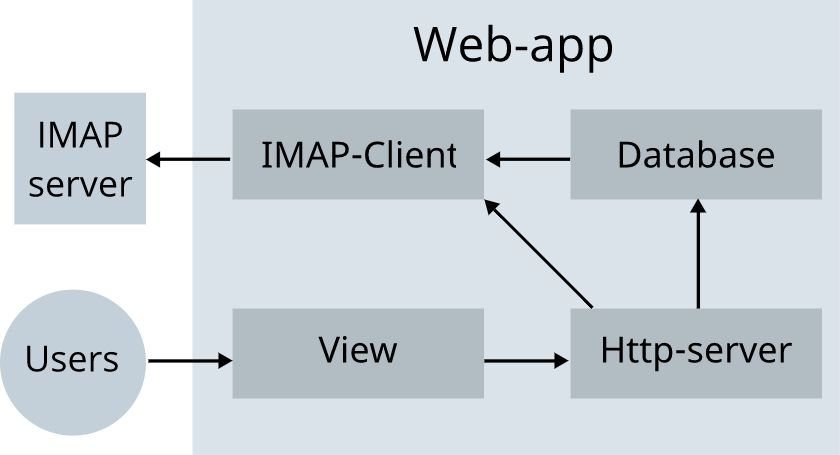
\includegraphics[scale=0.4]{pics/architecture}
            \caption{Компоненты приложения и связи между ними.}
            \label{architecture}
        \end{center}
    \end{figure}

    Таким образом, было решено создать веб-приложение, которое позволяет подключиться с помощью браузера
    и получить почтовые данные из указанного IMAP сервера.

\subsection{Поддерживаемые команды IMAP протокола}

    IMAP - Internet Message Access Protocol (RFC 3501), протокол прикладного уровня, предназначенный
    для приёма и управления электронной почтой размещенной на почтовом сервере.
    Базируется на транспортном протоколе TCP.

    IMAP работает только с сообщениями и не требует каких-либо пакетов со специальными заголовками.

    Каждое сообщение имеет несколько связанных с ним атрибутов. Несколько из них приведено ниже:

    
    \textbf{UID}

    Каждому сообщению на сервере ставится в соответствие 32-битный код, который при использовании совместно с уникальным
    идентификатором образует 64-битовую последовательность, гарантирующую однозначную идентификацию сообщения в почтовом ящике.


    \textbf{Порядковый номер сообщения}

    Порядковый номер сообщения в почтовом ящике начинается с 1.
    Каждое сообщение, начиная со второго, имеет порядковый номер ровно на 1 больше, чем предшествующее ему.

    Любая процедура начинается с команды клиента.
    Любая команда клиента начинается с префикса-идентификатора (обычно короткая буквенно-цифровая строка,
    например, A0001, A0002 и т. д.), называемого меткой. Для каждой команды клиент генерирует свою метку.

    
    Реализованный в рассматриваемом приложении IMAP клиент поддерживает следующие команды:

    
    \subsubsection{Login command}

        Команда $login$ предназначена для аутентификации пользователя на IMAP-сервере.

        \textbf{Аргументы:}  имя пользователя и пароль \\

        \textbf{Возможный ответ сервера:}

        OK - авторизация завершена

        NO - имя пользователя и пароль не совпадают

        BAD - неизвестная команда или некорректные аргументы \\


        \textbf{Пример использования:}  

        C: a001 LOGIN SMITH SESAME

        S: a001 OK LOGIN completed


    \subsubsection{Examine command}

        Команда $examine$ предназначена для выбора рабочей почтовой папки.
        Отличительной особенностю этой команды является то, что она открывает папку только на чтение.

        \textbf{Аргументы:}  имя почтовой папки \\

        \textbf{Возможный ответ сервера:}

        OK - почтовая папка успешно выбрана

        NO - такой почтовой папки не существует, не могу подключиться к почтовой папке

        BAD - неизвестная команда или некорректные аргументы \\


        \textbf{Пример использования:}  

        C: A932 EXAMINE blurdybloop

        S: * 17 EXISTS

        S: * 2 RECENT

        S: * OK [UNSEEN 8] Message 8 is first unseen

        S: * OK [UIDVALIDITY 3857529045] UIDs valid

        S: * OK [UIDNEXT 4392] Predicted next UID

        S: * FLAGS ($\textbackslash$ Answered $\textbackslash$ Flagged
        $\textbackslash$ Deleted $\textbackslash$ Seen $\textbackslash$ Draft)

        S: * OK [PERMANENTFLAGS ()] No permanent flags permitted

        S: A932 OK [READ-ONLY] EXAMINE completed

    \subsubsection{Select command}

        Команда $select$ предназначена для выбора рабочей почтовой папки.
        Команда открывает папку как на чтение, так и на запись в отличии от $examine$

        \textbf{Аргументы:}  имя почтовой папки \\

        \textbf{Возможный ответ сервера:}

        OK - почтовая папка успешно выбрана

        NO - такой почтовой папки не существует, не могу подключиться к почтовой папке

        BAD - неизвестная команда или некорректные аргументы \\


        \textbf{Пример использования:}  

        C: A142 SELECT INBOX

        S: * 172 EXISTS

        S: * 1 RECENT

        S: * OK [UNSEEN 12] Message 12 is first unseen

        S: * OK [UIDVALIDITY 3857529045] UIDs valid

        S: * OK [UIDNEXT 4392] Predicted next UID

        S: * FLAGS ($\textbackslash$ Answered $\textbackslash$ Flagged
        $\textbackslash$ Deleted $\textbackslash$ Seen $\textbackslash$ Draft)

        S: * OK [PERMANENTFLAGS ($\textbackslash$ Deleted $\textbackslash$ Seen $\textbackslash$ *)] Limited

        S: A142 OK [READ-WRITE] SELECT completed


    \subsubsection{Fetch command}

        Команда $fetch$ предназначена для получения сообщений.

        \textbf{Аргументы:}  макрос определяющий данные, которые необходимо получить \\

        \textbf{Возможный ответ сервера:}

        OK - данные успешно получены

        NO - не могу получить данные

        BAD - неизвестная команда или некорректные аргументы \\


        \textbf{Пример использования:}  

        C: A654 FETCH 2:4 (FLAGS BODY[HEADER.FIELDS (DATE FROM)])

        S: * 2 FETCH ....

        S: * 3 FETCH ....

        S: * 4 FETCH ....

        S: A654 OK FETCH completed


    \subsubsection{Search command}

        Команда $search$ предназначена для поиска сообщений по заданным критериям.
        Возвращает номера писем, соответствующих условию поиска.

        \textbf{Аргументы:}  критерий поиска \\

        \textbf{Возможный ответ сервера:}

        OK - поиск успешно завершен

        NO - ошибка поиска

        BAD - неизвестная команда или некорректные аргументы \\


        \textbf{Пример использования:}  

        C: A282 SEARCH FLAGGED SINCE 1-Feb-1994 NOT FROM "Smith"

        S: * SEARCH 2 84 882

        S: A282 OK SEARCH completed

        C: A283 SEARCH TEXT "string not in mailbox"

        S: * SEARCH

        S: A283 OK SEARCH completed

        C: A284 SEARCH CHARSET UTF-8 TEXT {6}

        C: XXXXXX

        S: * SEARCH 43

        S: A284 OK SEARCH completed


    \subsubsection{List command}

        Команда $list$ предназначена для вывода
        списка папок, расположенных на IMAP-сервере
        и соответствующих условиям поиска.

        \textbf{Аргументы:}  критерий поиска \\

        \textbf{Возможный ответ сервера:}

        OK - список успешно составлен

        NO - не могу составить список

        BAD - неизвестная команда или некорректные аргументы \\


        \textbf{Пример использования:}  

        C: A101 LIST "{}"{} "{}"{}
        
        S: * LIST ($\textbackslash$Noselect) "/" "{}"{}

        S: A101 OK LIST Completed

        C: A102 LIST \# news.comp.mail.misc "{}"

        S: * LIST ($\textbackslash$Noselect) "."{} \# news.

        S: A102 OK LIST Completed

        C: A103 LIST /usr/staff/jones "{}"

        S: * LIST ($\textbackslash$Noselect) "/" /

        S: A103 OK LIST Completed

        C: A202 LIST \textasciitilde/Mail/ \%

        S: * LIST ($\textbackslash$Noselect) "/"{} \textasciitilde/Mail/foo

        S: * LIST () "/"{} \textasciitilde/Mail/meetings

        S: A202 OK LIST completed


    \subsubsection{Logout command}

        Команда $logout$ предназначена для завершения обмена данными между IMAP-клиентом и IMAP-сервером.

        \textbf{Аргументы:}  отсутствуют \\

        \textbf{Возможный ответ сервера:}

        OK - успешно завершение сессии

        BAD - неизвестная команда или некорректные аргументы \\


        \textbf{Пример использования:}

        C: A023 LOGOUT

        S: * BYE IMAP4rev1 Server logging out

        S: A023 OK LOGOUT completed

        (Server and client then close the connection)


\subsection{Графический интерфейс приложения}

    На рисунках \ref{login}, \ref{spam}, \ref{letter} представлен графический интерфейс приложения.

    \begin{figure}[H]
        \begin{center}
            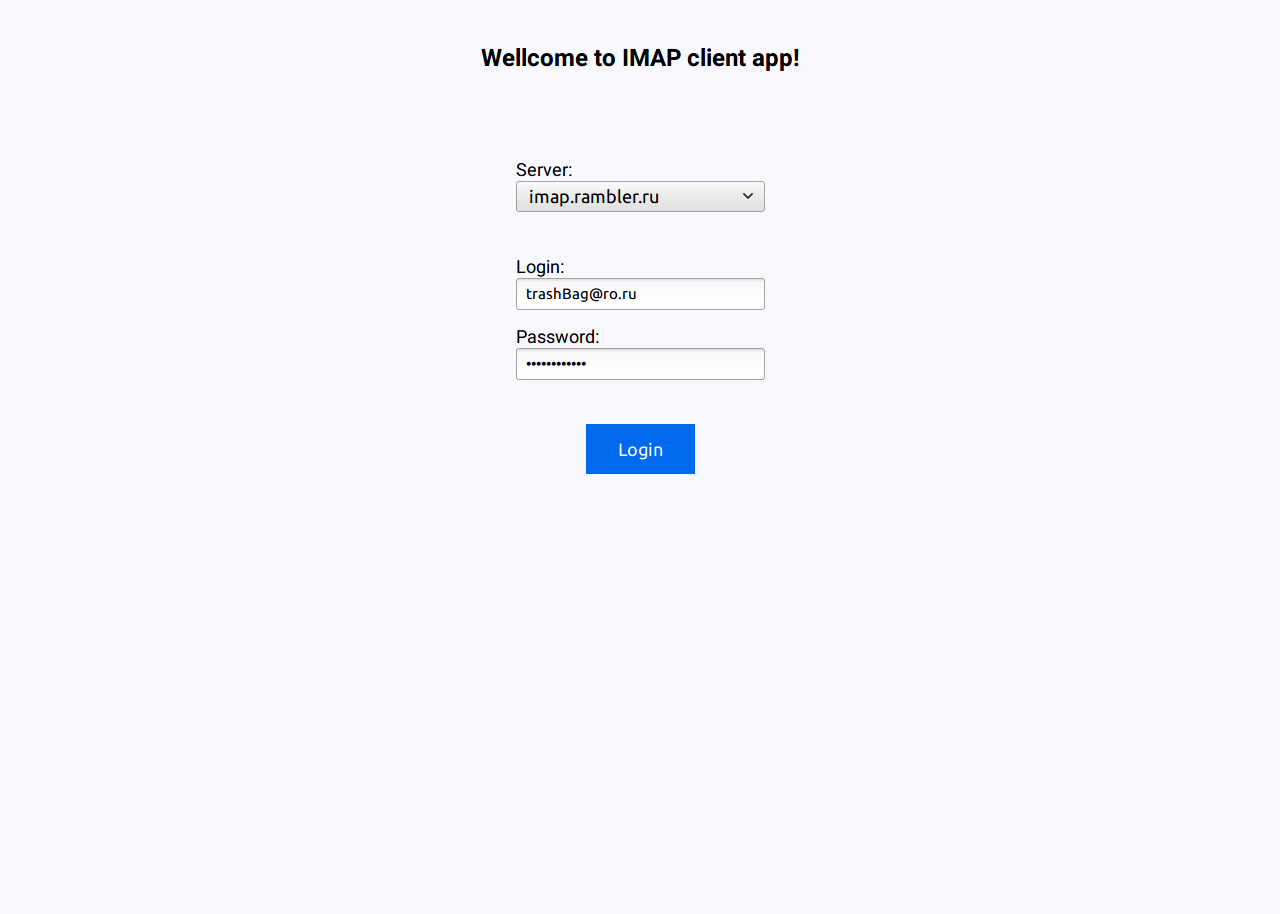
\includegraphics[scale=0.25]{pics/login}
            \caption{Графический интерфейс приложения. Окно логина.}
            \label{login}
        \end{center}
    \end{figure}

    \begin{figure}[H]
        \begin{center}
            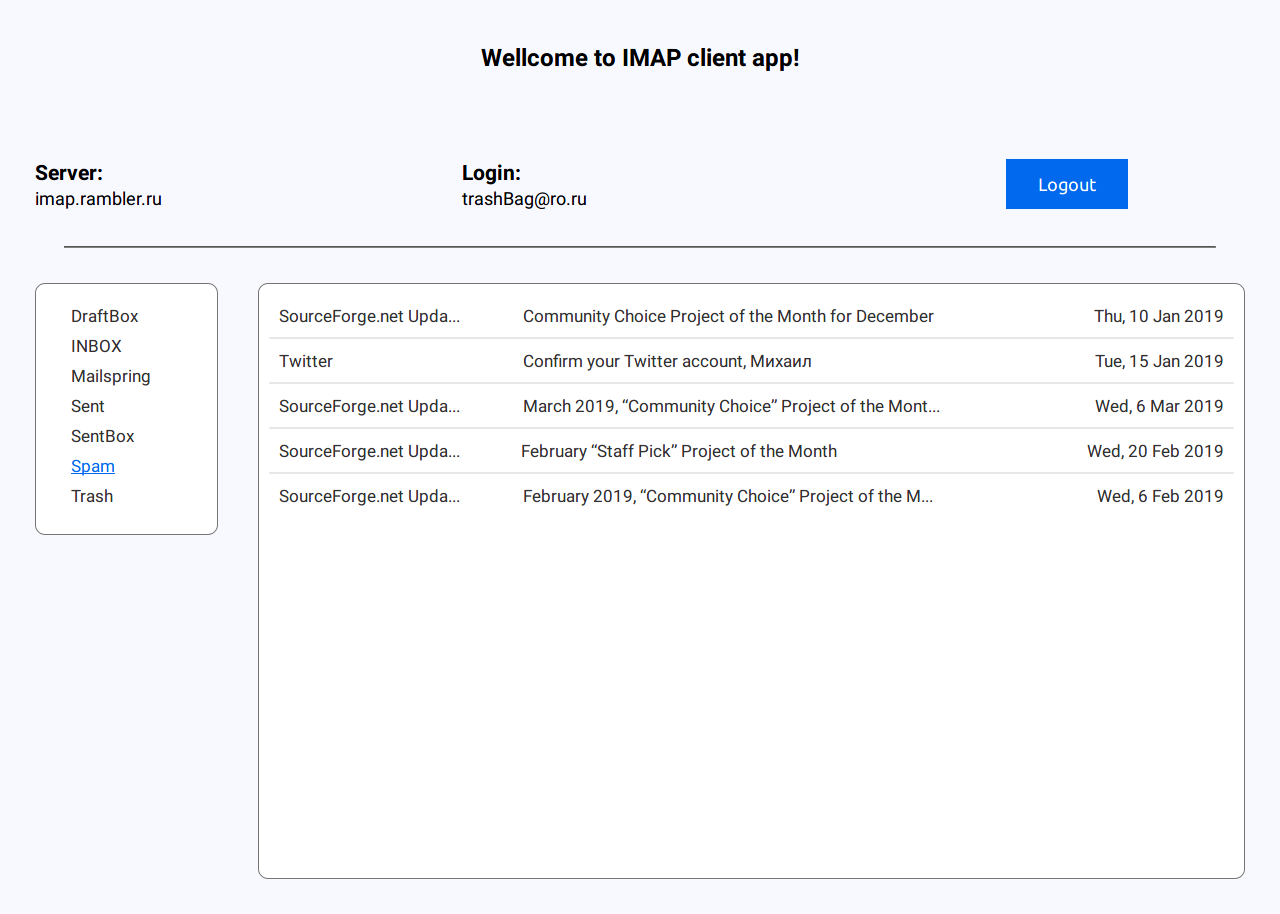
\includegraphics[scale=0.4]{pics/spam}
            \caption{Графический интерфейс приложения. Открыта папка Spam.}
            \label{spam}
        \end{center}
    \end{figure}

    \begin{figure}[H]
        \begin{center}
            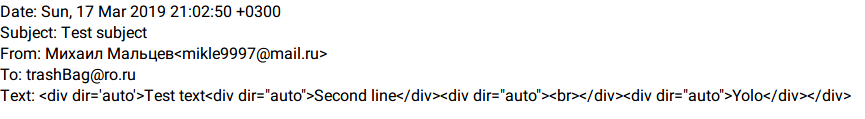
\includegraphics[scale=0.55]{pics/letter}
            \caption{Графический интерфейс приложения. Отображение письма.}
            \label{letter}
        \end{center}
    \end{figure}

    Разработанный интерфейс отображает используемую, на данный момент,
    почтовую папку и выделяет непрочитанные сообщения.
    Окно логина уведомляет в случае, если пользователь забыл ввести данные в одну из форм
    или он ввёл некорректные данные. При открытие письмо выглядит максимально минималистично.
    На отдельные строчки вынесены такие поля, как дата, тема письма, от кого оно, кому предназначалось и собственно сам текст письма.

\subsection{Тестирование}

    Для тестирования был выбран действующий почтовый сервер - imap.rambler.ru. Приложение подключалось к серверу imap.rambler.ru по порту 993.
    С сервера извлекались почтовые данные, которые успешно отображались приложением. Также был проведен эксперимент с посылкой нового письма
    на сервер, с помощью стороннего сервиса, и отображением его в разработаном приложении. Все проверки были успешно пройдены.

\section{Вывод}

    В результате выполнения работы был создан IMAP-клиент. 
    В процессе создания приложения был подробно изучен протокол IMAP и были закреплены знания, принципов функционирования почтовых сервисов.
    Также, в связи с тем, что данные приходящие от почтового сервиса требовалось в понятном виде продемонстрировать пользователю,
    были улучшены навыки работы с регулярными выражениями.
    Разработанное приложение было протестировано в работе с реальным IMAP-сервером, тестирование подтвердило работоспособность.

\newpage

\section{Листинги}

    \lstinputlisting{../main.go}
    \lstinputlisting{../db/db.go}
    \lstinputlisting{../imap/client.go}
    \lstinputlisting{../imap/commands.go}
    \lstinputlisting{../imap/parsers.go}
    \lstinputlisting{../imap/read.go}
    \lstinputlisting{../imap/utils.go}

    \lstinputlisting{../templates/content.html}
    \lstinputlisting{../templates/footer.html}
    \lstinputlisting{../templates/header.html}
    \lstinputlisting{../templates/index.html}
    \lstinputlisting{../templates/letter.html}

    \lstinputlisting{../public/main.css}
    \lstinputlisting{../public/main.js}

\end{document}